% In this chapter discuss functional requirements
% This is worth a lot so let's nail it
\chapter{Functional Requirements Specification}


% Who has a stake in the project?
% IE prospective users, possibly the finance
% backend people, possibly companies...
\section{Stakeholders}

As identified previously, the primary parties interested in
this platform would be students and novice investors. However,
due to the popularity of related platforms, it is not
unrealistic that a future incarnation of this application 
could be marketed actively towards target groups. For instance,
students would be promoted to this service to host various
competitions; introductory texts on finance could also place
references here. To that end, it behooves us to cater to those
primary demographics.

At the same time, gaining a sufficient user base would also
open the possibility of discreetly placed advertisements 
throughout the application. Therefore, we can consider 
marketing agents to be stakeholders as well, with the caveat
that the site will not initially be designed with commercial
product placement in mind. Our decision reflects a popular 
business model for firms today, in which an easily monetizable
application does not compromise its rollout with commercials
which can easily be implemented later. Yet another reason is 
the consideration of the various business expenses associated 
with a commercial rollout -- notably the licenses and fees
associated with having a commercial (as opposed to free)
service. % no typos here...

% Who are some actors and what are their goals?
% I'm filling this from Nick's use cases
% but there could be even more
% Probably include a new file 
\section{Actors and Goals}

\subsection{Guest}
An unregistered visitor or a visitor who is not logged in.
\begin{itemize}
\item[--] Create an account
\item[--] View top users and stocks
\end{itemize}
\subsection{User}
A visitor who has registered and logged in to an account.
\begin{itemize}
\item[--] Join/create leagues
\item[--] Take part in competitions
\item[--] Change personal settings
\end{itemize}
\subsection{League Manager}
A user who created or controls a league.
\begin{itemize}
\item[--] Create a league competition
\item[--] Edit league settings
\end{itemize}
\subsection{Site Administrator}
A user who can control key aspects of the site
\begin{itemize}
\item[--] Change global settings
\item[--] Create/edit global events
\item[--] View statistics of site
\end{itemize}
\subsection{Database}
The unit that holds information about all users' data.
\begin{itemize}
\item[--] Push data back to views about users/events
\item[--] Store new data about about users/events
\end{itemize}
\subsection{Financial API}
The unit that knows about current financial 
\begin{itemize}
\item[--] Retrieve data about stocks
\end{itemize}


\begin{figure}
\centering
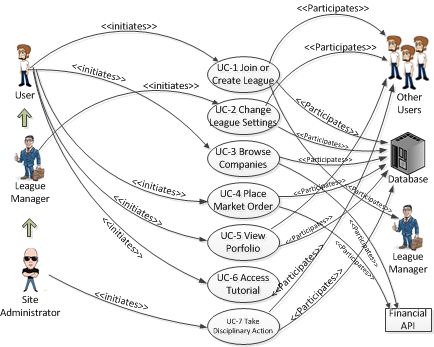
\includegraphics[width=5.5in]{./Diagrams/UseCaseDiagram.png}
\caption{This graphic illustrates the relationships between the core actors of our platform.}
\end{figure}

% This is for the use cases
% These take up a lot so should be in another file
\section{Use Cases}

% This file contains only the fully dressed use cases

Before a user can participate in most of the functionality of our site, the user must first join or create a league. Ultimately, creating a league is very similar to joining a league, with the only exception being that the user becomes League Manager of a league that they create and that the new league must be added to the database. Therefore, the two will be represented as one use case with alternate scenarios. The responsibilities of the League Manager will be explored in a later use case. One relevant aspect of the responsibily of a League Manager to the use case though, is whether a league is made public or private; that is, whether it shows up in a public league listing page or can only be joined by direct invitiation from the League Manager. Thus, our first use case involves a business policy: \\ \\
\textbf{CG-BP01:} So that a user may create a join leagues with only their friends, leagues marked as private will not show up on the league listings. \\

Thus, a user will only be able to browse listings of public leagues. \\

\begin{centering}
\renewcommand\arraystretch{1.3} % Causes rows to be spaced
\begin{longtable}{|p{1.2in} p{5in}|}
\hline
% BFSeries should cause text to be bold
% Color1 should cause text to be blue... may be broken idk
\bfseries{\color{color1}Use Case UC-1} & \bfseries{\color{color1}Join League} \\
\hline
Related Requirements: & ST-2, ST-21 \\ 
Initiating Actor:     & User \\
Actor's Goal:         & To join or create a fantasy finance league \\
Participating Actors:  & Database, Other Users, League Managers\\
Preconditions:        & -A public league exists and has open positions \\
 & -User is logged in \\
Postconditions:       & -The \textbf{Database} is updated to reflect the user's participation in the lague \\
\hline
\multicolumn{2}{|c|}{\color{color1}Flow of Events for Main Success Scenario:}\\
\hline
$\rightarrow$ & 1. \textbf{User} navigates to leagues listing page \\
$\leftarrow$ & 2. \textbf{System} displays public leagues available for the \textbf{User}, sorted by date created \\
$\rightarrow$ & 3. \textbf{User} selects join on a league in which they are interesting in joining \\
$\leftarrow$ & 4. \textbf{System} registers \textbf{User} into that league, notifying \textbf{Database} to update to reflect this change \\
\hline
\multicolumn{2}{|c|}{\color{color1}Flow of Events for Extensions (Alternate Scenarios):} \\
\hline
\multicolumn{2}{|p{6.2in}|}{3a. The \textbf{user} selects create league rather than join league} \\
\hline
$\rightarrow$ & 1.  \textbf{User} inputs desired league name and settings \\
$\leftarrow$ & 2. \textbf{System} (a) creates the league and inputs it to the \textbf{Database} and (b) registers the \textbf{User} into that league as \textbf{League Manager} \\
\hline 
\end{longtable}
\end{centering}

It is important here to note another business policy of our site relevant to the user's experience: \\ \\
\textbf{CG-BP02:} A user is able to join an unlimited number of leagues and become League Manager for as many leagues as the user wishes to create. \\

Though the settings are selected when creating the league, any League Manager can change the settings of their league at any time. These settings are comprehensive, including such items as name, privacy, number of spots, and rules which define how much money each league member receives to spend and other conditions under which all league members much operate for participation in that league. In addition, the League Manager can also manage members from the settings.\\

\begin{centering}
\renewcommand\arraystretch{1.3} % Causes rows to be spaced
% p{} causes text wrapping effects for longer
% columns
\begin{longtable}{|p{1.2in} p{5in}|}
\hline
% BFSeries should cause text to be bold
% Color1 should cause text to be blue... may be broken idk
\bfseries{\color{color1}Use Case UC-2} & \bfseries{\color{color1}Change League Settings} \\
\hline
Related Requirements: & ST-22, ST-23\\ 
Initiating Actor:     & League Manager \\
Actor's Goal:         & To change the settings of a league and manage its members \\
Participating Actors:  & Database, other Users \\
Preconditions:        & -User is the League Manager of the league \\
 & -User is logged in \\
Postconditions:       & -The league settings have been changed as desired and the \textbf{Database} reflects the changes \\
\hline
\multicolumn{2}{|c|}{\color{color1}Flow of Events for Main Success Scenario:}\\
\hline
$\rightarrow$ & 1. \textbf{League Manager} selects the league settings option from the league page \\
$\leftarrow$ & 2. \textbf{System} requests the current settings from the \textbf{Database} and presents them to the \textbf{League Manager} along with options to change the settings \\
$\rightarrow$ & 3. \textbf{League Manager} updates the settings, such as privacy, league name, number of spots, rules, and managing users \\
$\leftarrow$ & 4. \textbf{System} sends the updated settings to the \textbf{Database} \\
\hline
\multicolumn{2}{|c|}{\color{color1}Flow of Events for Extensions (Alternate Scenarios):} \\
\hline
\multicolumn{2}{|p{6.2in}|}{1a. The \textbf{User} selecting league settings is not the \textbf{League Manager}} \\
\hline
$\leftarrow$ & 1. \textbf{System} requests the current settings from the \textbf{Database} and displays them, but does not provide ways to change them \\
\hline
\multicolumn{2}{|p{6.2in}|}{4a. The \textbf{League Manager} has altered the status of a league member} \\
\hline
$\leftarrow$ & 1. \textbf{System} will request the \textbf{Database} to update the \textbf{User}'s status in the league, be it becoming league manager or removing that \textbf{User}'s instance from this league (banned)\\
\hline
\end{longtable}
\end{centering}

It is of some concern that League Managers may become abusive of their powers, and therefore it is important to create on a policy to explicitly state how this power is treated. In modern fantasy leagues (such as football, baseball, etc.), the League Manager does not typically have their power moderated, and this has not caused any problems in the success of these fantasy websites. The ability to leave a league and join another is left to the users if they feel that their league manager has become abusive. Their joining of the league acts as an implicit contract to accept of the League Manager's settings. However, if this League Manager becomes a problem and users bring it to an administrator's attention, disciplinary action may be taken. Thus we generate the next site policy:\\ \\
\textbf{CG-BP03:} A League Manager is able to change the status of users in their league without moderation. However, if a League Manager is deemed abusive, a site administrator may take disciplinary action against them. \\

Core to our site is the ability of the user to have access to information about companies so that the user may make informed decisions on how he would like to invest. As this is so crucial to the functionality of this project, it is absolutely necessary to make information easily available to the user and presented in a way that is clear and easy to understand. Therefore, the search of companies as mentioned in ST-3 should be simple to use and intuitive and the display of company profiles as mentioned in ST-4 should be such that a user can easily access any desired information about the company's financial performance. \\

% The following is a worked example. Copy/Paste this format
% and you should survive...
\begin{centering}
\renewcommand\arraystretch{1.3} % Causes rows to be spaced
% p{} causes text wrapping effects for longer
% columns
\begin{longtable}{|p{1.2in} p{5in}|}
\hline
% BFSeries should cause text to be bold
% Color1 should cause text to be blue... may be broken idk
\bfseries{\color{color1}Use Case UC-3} & \bfseries{\color{color1}Browse Companies} \\
\hline
Related Requirements: & ST-3, ST-4 \\ 
Initiating Actor:     & User \\
Actor's Goal:         & To bring up information on a desired company \\
Participating Actors:  & Database, Financial API \\
Preconditions:        & -Financial API is accepting inquiries \\
 & -User is logged in \\
Postconditions:       & -None worth mentioning \\
\hline
\multicolumn{2}{|c|}{\color{color1}Flow of Events for Main Success Scenario:}\\
\hline
$\rightarrow$ & 1. \textbf{User} begins entering a search term \\
$\leftarrow$ & 2. \textbf{System} makes suggestions for companies in real-time \\
$\rightarrow$ & 3. \textbf{User} enters search term or selects a suggestion \\
$\leftarrow$ & 4. \textbf{System} (a) requests information from \textbf{Financial API} and (b) displays the information to the user in a clear and interactive manner \\
\hline
\multicolumn{2}{|c|}{\color{color1}Flow of Events for Extensions (Alternate Scenarios):} \\
\hline
\multicolumn{2}{|p{6.2in}|}{1a. The \textbf{User} selects a direct link to a company rather than enter a search term} \\
\hline
$\leftarrow$ & 1.  Same as step 4 above \\
\hline 
\multicolumn{2}{|p{6.2in}|}{3a. The search term is invalid, i.e. the company does not exist} \\
\hline
$\leftarrow$ & 1.  System informs user company does not exist and offers similarly titled companies as links \\
\hline
\end{longtable}
\end{centering}

Note that the exact way in which the information requested from the Financial API is displayed to the user is not specified in this use case. This will be described instead in later sections about on-screen appearance requirements as to try to separate the functionality of the site and design of the site as separate as possible. \\

The goal of browsing companies ultimately is for the user to gain the knowledge needed to place market orders. Market orders are the atomic action of our site; i.e. the center point of every league is the user's ability to initiate transactions in an attempt to invest their money as best they can. \\

\begin{centering}
\renewcommand\arraystretch{1.3} % Causes rows to be spaced
\begin{longtable}{|p{1.2in} p{5in}|}
\hline
% BFSeries should cause text to be bold
% Color1 should cause text to be blue... may be broken idk
\bfseries{\color{color1}Use Case UC-4} & \bfseries{\color{color1}Place Market Order} \\
\hline
Related Requirements: & ST-5 \\ 
Initiating Actor:     & User \\
Actor's Goal:         & To buy or sell stock, or to place a short, stop, or limit order \\
Participating Actors:  & Database, Financial API \\
Preconditions:        & -Financial API is accepting inquiries \\
 & -User is logged in \\
 & -User is a member of a league \\
Postconditions:       & -\textbf{User}'s portfolio is updated to reflect change in position \\
\hline
\multicolumn{2}{|c|}{\color{color1}Flow of Events for Main Success Scenario:}\\
\hline
$\rightarrow$ & 1. \textbf{User} selects the league in which they would like to place the order \\
$\leftarrow$ & 2. \textbf{System} displays prompt for market order, including type, amount, and company \\
$\rightarrow$ & 3. \textbf{User} fills out form and requests the order be placed \\
$\leftarrow$ & 4. \textbf{System} (a) requests market price from \textbf{Financial API} and (b) places the order into the \textbf{Database} \\
$\leftarrow$ & 5. The order either resolves or expires, and the \textbf{System} updates the \textbf{User}'s position in the \textbf{Database} accordingly \\
\hline
\multicolumn{2}{|c|}{\color{color1}Flow of Events for Extensions (Alternate Scenarios):} \\
\hline

\multicolumn{2}{|p{6.2in}|}{1a. The \textbf{User} chooses to place a market order from a company's profile rather than from the league page} \\
\hline
$\rightarrow$ & 1. The \textbf{User} selects which league in which to place the order  \\
$\leftarrow$ & 2. The \textbf{System} takes the \textbf{User} to league marker order prompt as described in Step 2 above, with the prompt for company already filled out \\
$\rightarrow$ & 3. Go to Step 3 above \\
\hline
\multicolumn{2}{|p{6.2in}|}{4a. The \textbf{User} does not have enough money or margin to place the order} \\
\hline
$\leftarrow$ & 1. The \textbf{System} informs the \textbf{User} that they do not have enough money or margin to place the order and returns them to the market order prompt \\
\hline 
\end{longtable}
\end{centering}

The potential kinds of orders referenced in the above use case are defined in the glossary. The details on the necessary computations to enact these orders will be defined in a section later on. \\

In order to keep track of their own finances and any of their fellow league member's finances, a user must be able to view member portfolios. This keeps with the competitive nature of our site in addition to allowing the user to track their own progress. \\

\begin{centering}
\renewcommand\arraystretch{1.3} % Causes rows to be spaced
% p{} causes text wrapping effects for longer
% columns
\begin{longtable}{|p{1.2in} p{5in}|}
\hline
% BFSeries should cause text to be bold
% Color1 should cause text to be blue... may be broken idk
\bfseries{\color{color1}Use Case UC-5} & \bfseries{\color{color1}View Portfolio} \\
\hline
Related Requirements: & ST-6, ST-7, ST-11 \\ 
Initiating Actor:     & User \\
Actor's Goal:         & To view one's own finances or another's finances \\
Participating Actors:  & Database, other Users \\
Preconditions:        & -User is a member of a league \\
 & -User is logged in \\
 & -Database is tracking user's position \\
Postconditions:       & -None worth mentioning \\
\hline
\multicolumn{2}{|c|}{\color{color1}Flow of Events for Main Success Scenario:}\\
\hline
$\rightarrow$ & 1. \textbf{User} selects a league member's profile \\
$\leftarrow$ & 2. \textbf{System} requests that member's information from the \textbf{Database} and displays it in an organized and graphical manner to the \textbf{User} \\
\hline
\multicolumn{2}{|c|}{\color{color1}Flow of Events for Extensions (Alternate Scenarios):} \\
\hline
\multicolumn{2}{|p{6.2in}|}{2a. The \textbf{User} is viewing their own portfolio} \\
\hline
$\leftarrow$ & 1.  The \textbf{System} gives the \textbf{System} options to place market orders related to their existing positions \\
\hline
\end{longtable}
\end{centering}

Once again, the exact display of information is not defined in the use case, but rather will be explored further in the section about user interface specifications. Next to discuss is the tutorial as referenced in ST-8. We consider this to be one of the main aspects that separates us from previous iterations of fantasy stock leagues; our site will educate users new to finance and enable them to learn all about the world of finance and how to invest, in addition to how to these subjects relate to the use of our site.\\

\begin{centering}
\renewcommand\arraystretch{1.3} % Causes rows to be spaced
% p{} causes text wrapping effects for longer
% columns
\begin{longtable}{|p{1.2in} p{5in}|}
\hline
% BFSeries should cause text to be bold
% Color1 should cause text to be blue... may be broken idk
\bfseries{\color{color1}Use Case UC-6} & \bfseries{\color{color1}Access Tutorials} \\
\hline
Related Requirements: & ST-8 \\ 
Initiating Actor:     & User \\
Actor's Goal:         & To become educated in finance \\
Participating Actors:  & None \\
Preconditions:        & -User is logged in \\
Postconditions:       & -None worth mentioning \\
\hline
\multicolumn{2}{|c|}{\color{color1}Flow of Events for Main Success Scenario:}\\
\hline
$\rightarrow$ & 1. \textbf{User} selects the tutorial option from the site's main page \\
$\leftarrow$ & 2. \textbf{System} displays possible topics on which the \textbf{User} may be educated on \\
$\rightarrow$ & 3. \textbf{User} selects topic \\
$\leftarrow$ & 4. \textbf{System} presents an interactive tutorial to the \textbf{User}, which will be further elaborated upon in a later section \\
\hline
\end{longtable}
\end{centering}

In order to maintain a clean fantasy finance experience for our regular users, site administrators will reserve the ability to moderate other users--issuing warnings, suspensions, or even bans for abusive activity. To put it explicitly: \\
\textbf{CG-BP04:} Site administrators will warn, suspend, or ban users for abusive activity--this includes aggressive behavior on league comments or user messages, spamming users, joining numerous leagues without active participation, and anything else that is deemed to harm the experience for other users. \\


\begin{centering}
\renewcommand\arraystretch{1.3} % Causes rows to be spaced
% p{} causes text wrapping effects for longer
% columns
\begin{longtable}{|p{1.2in} p{5in}|}
\hline
% BFSeries should cause text to be bold
% Color1 should cause text to be blue... may be broken idk
\bfseries{\color{color1}Use Case UC-7} & \bfseries{\color{color1}Take Disciplinary Action} \\
\hline
Related Requirements: & ST-27 \\ 
Initiating Actor:     & Site Administrator \\
Actor's Goal:         & To take action against an abusive \textbf{User} \\
Participating Actors:  & Database, Users \\
Preconditions:        & -Initiating actor is a \textbf{Site Administrator} \\
 & -There are outstanding abuse reports \\
Postconditions:       & -The \textbf{Database} is updated to reflect any actions taken against the \textbf{User} \\
 & The abuse report shows that it has been resolved on the administration page\\
\hline
\multicolumn{2}{|c|}{\color{color1}Flow of Events for Main Success Scenario:}\\
\hline
$\rightarrow$ & 1. \textbf{Site Administrator} selects the site administration page option from the main screen (only viewable by \textbf{Site Administrators}) \\
$\leftarrow$ & 2. \textbf{System} makes a request to the \textbf{Database} and displays all outstanding abuse reports\\
$\rightarrow$ & 3. \textbf{Site Administrator} (a) selects an abuse report, (b) reviews the report, and (c) selects what action is to be taken (if any)\\
$\leftarrow$ & 4. \textbf{System} implements the action selected by the \textbf{Site Administrator} and updates the \textbf{Database} accordingly \\
\hline
\end{longtable}
\end{centering}


\section{System Sequence Diagrams}

\begin{figure}
\centering
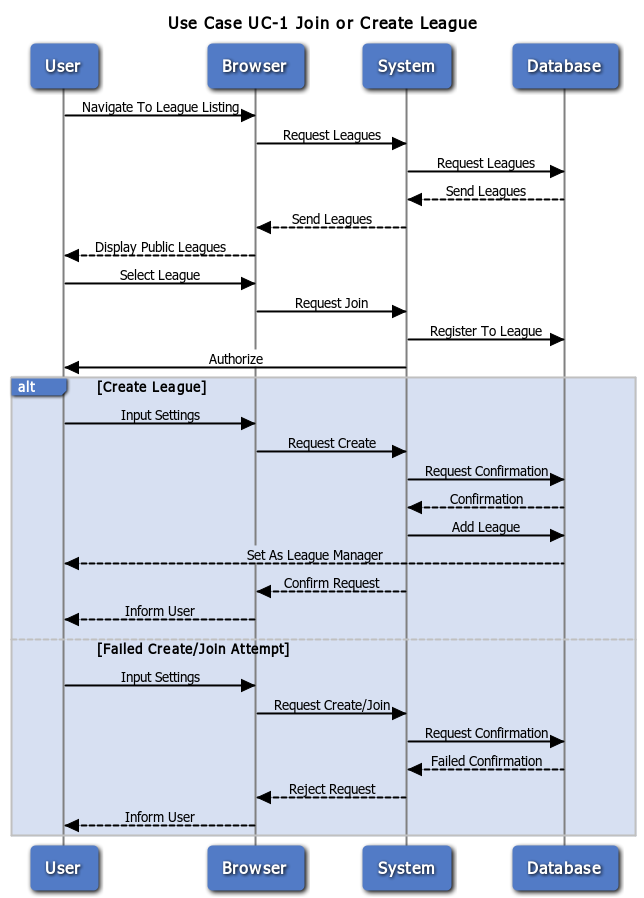
\includegraphics[width=5.5in]{./Diagrams/SystemSequenceDiagrams/uc1.png}
\caption{Sequence Diagram for UC-1 on page \pageref{UC-1}}
\end{figure}

\begin{figure}
\centering
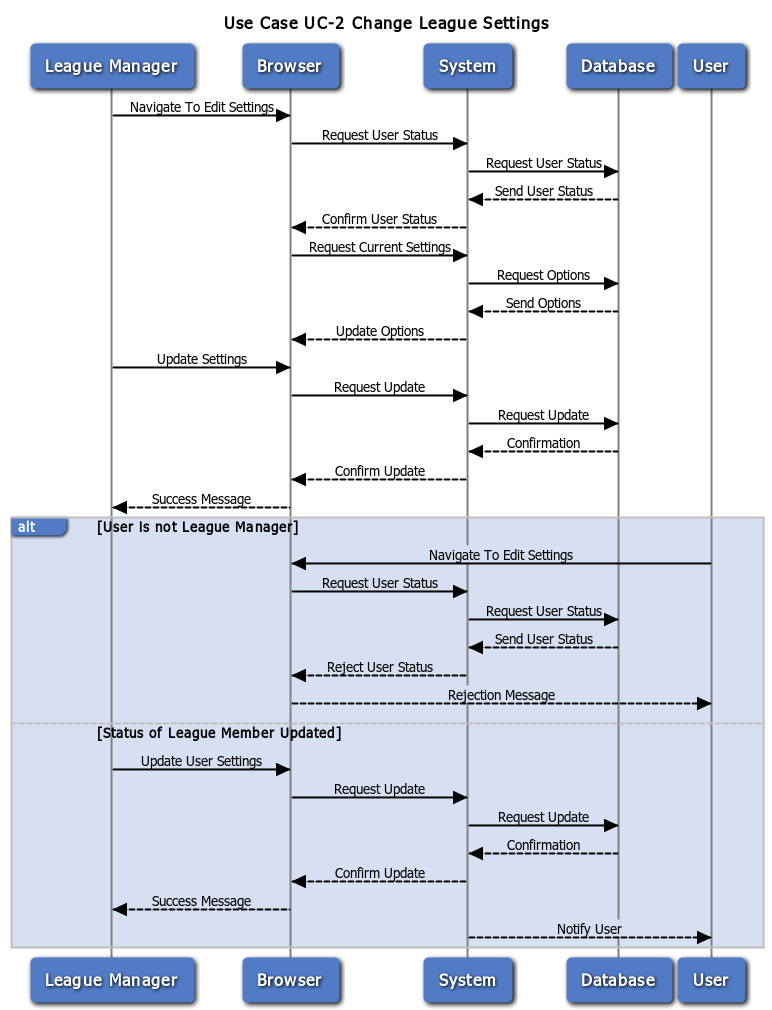
\includegraphics[width=5.5in]{./Diagrams/SystemSequenceDiagrams/uc2.png}
\caption{Sequence Diagram for UC-2 on page \pageref{UC-2}}
\end{figure}

\begin{figure}
\centering
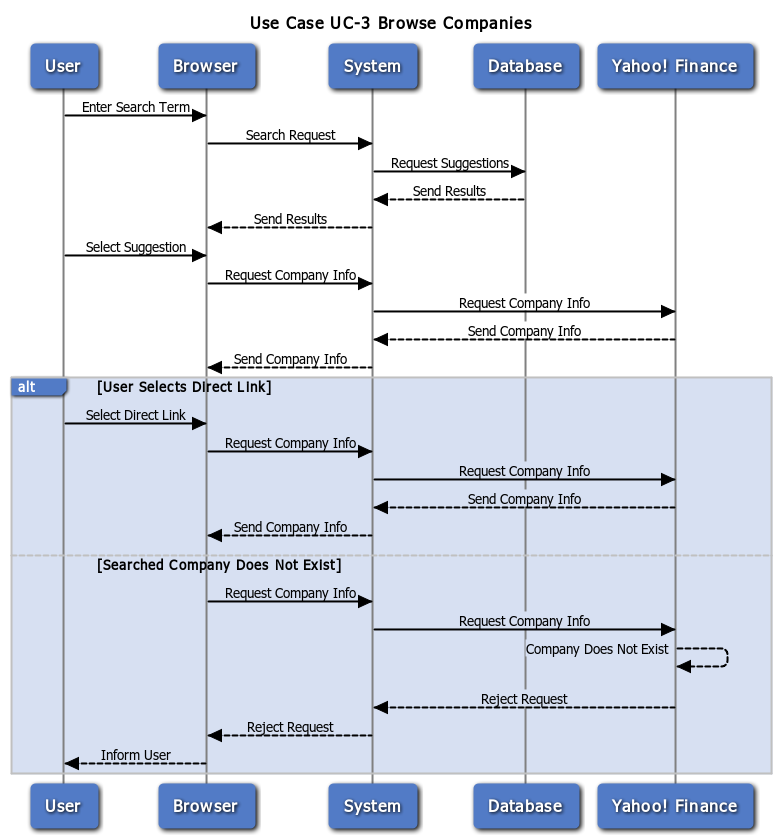
\includegraphics[width=5.5in]{./Diagrams/SystemSequenceDiagrams/uc3.png}
\caption{Sequence Diagram for UC-3 on page \pageref{UC-3}}
\end{figure}

\begin{figure}
\centering
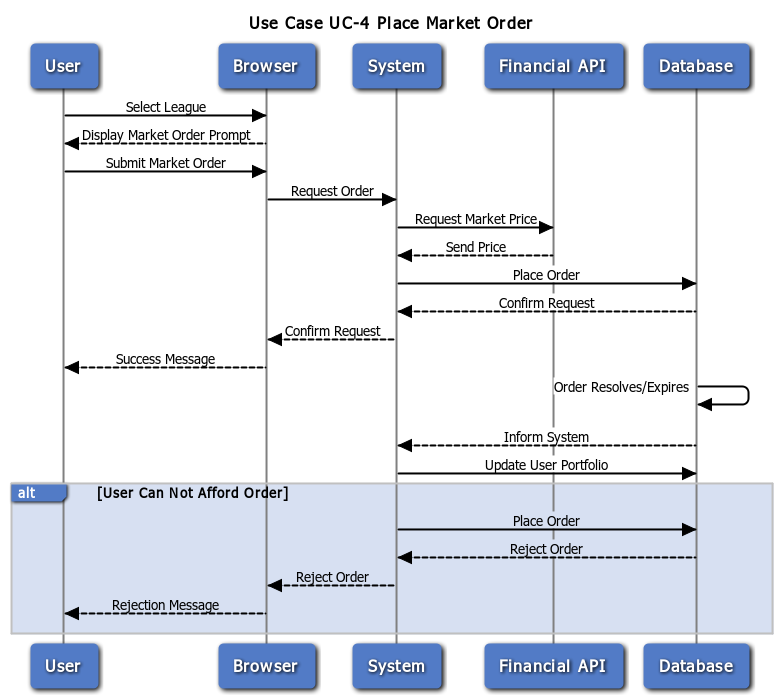
\includegraphics[width=5.5in]{./Diagrams/SystemSequenceDiagrams/uc4.png}
\caption{Sequence Diagram for UC-4 on page \pageref{UC-4}}
\end{figure}

\begin{figure}
\centering
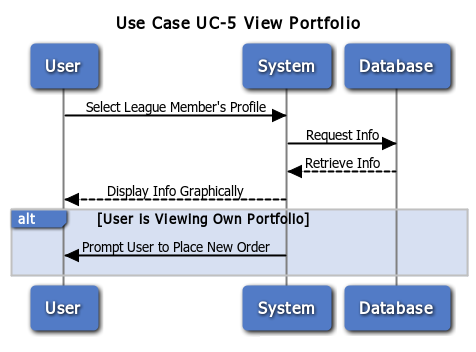
\includegraphics[width=5.5in]{./Diagrams/SystemSequenceDiagrams/uc5.png}
\caption{Sequence Diagram for UC-5 on page \pageref{UC-5}}
\end{figure}

\begin{figure}
\centering
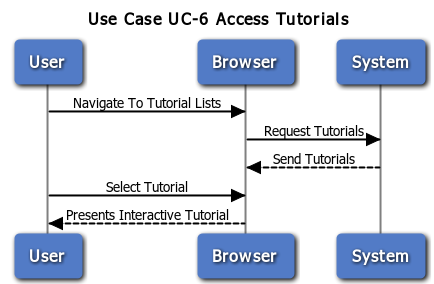
\includegraphics[width=5.5in]{./Diagrams/SystemSequenceDiagrams/uc6.png}
\caption{Sequence Diagram for UC-6 on page \pageref{UC-6}}
\end{figure}

\begin{figure}
\centering
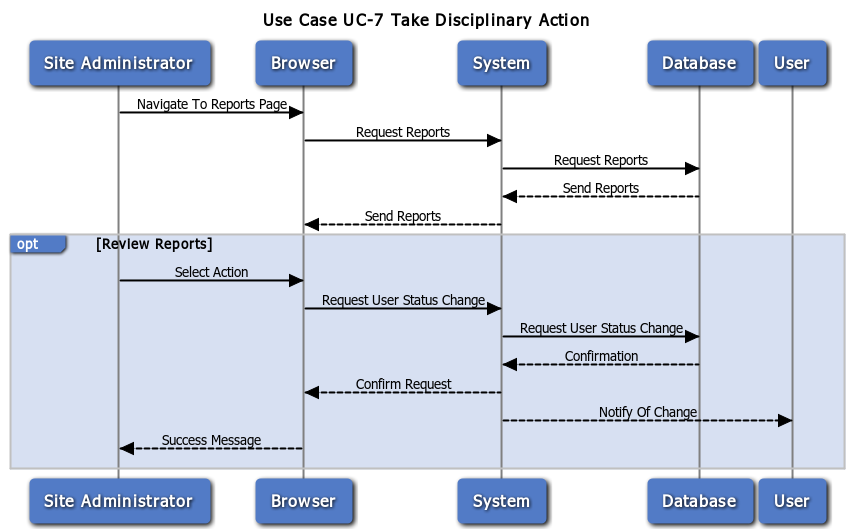
\includegraphics[width=5.5in]{./Diagrams/SystemSequenceDiagrams/uc7.png}
\caption{Sequence Diagram for UC-7 on page \pageref{UC-7}}
\end{figure}